\section{Initial Tree Construction Process}
\label{MCRP}
\subsection{Details of MCRP}

WSNs often suffer from frequent occurrences of external interference such as Wi-Fi and Bluetooth.
Multichannel communications in wireless networks can alleviate the effects of interference to enable WSNs to operate reliably in the presence of such interference. As a result, multichannel solution can improve the network efficiency of spectrum usage, network stability, link reliability, minimise latency and minimise the number of packet loss, hence, retransmission.

Multichannel Cross-Layer Routing Protocol (MCRP) \cite{mcrp} is a decentralised cross-layer protocol with a centralised controller. The cross layer multichannel protocol focuses on the network and application layers. This allows channel assignment decisions to be made without being limited by the low layer complexity. The system has two parts: a central algorithm which is typically run by the LPBR for nodes channel allocation; and a protocol which allows the network to communicate the channel change decision, probe the new channel and either communicate the success of the change or fall back to the previous channel. MCRP concentrates on finding channels for the nodes that are free from or have low external interference to maximise the packet reception rate. It also allows the allocation of these channels to avoid cross interference between different pairs of nodes.


%minimise the chances of nodes which are physically near to communicate on the same channel. Hence, it reduces cross interference between different pairs of nodes, external interference and maxim.

%This chapter introduces MCRP, a multichannel cross layer routing protocol that jointly optimise the network communications through channel decisions from the application, network and MAC layers. It uses a centralised controller for nodes channel allocation. The channel condition is tested through probing packets during run time as it varies depending on the location, time and usage. By doing so, the nodes would use less interference channels for communications to maximise the packet reception rate. MCRP uses a two-hop colouring strategy to avoid nearby nodes from competing to transmit on the same channel at the same time and internal interference that could occur. In order to allow reconnection and new nodes to join an existing topology, RPL control messages are adjusted to support multichannel. 

\subsubsection{Initialisation}
%\begin{figure}
%\centering
%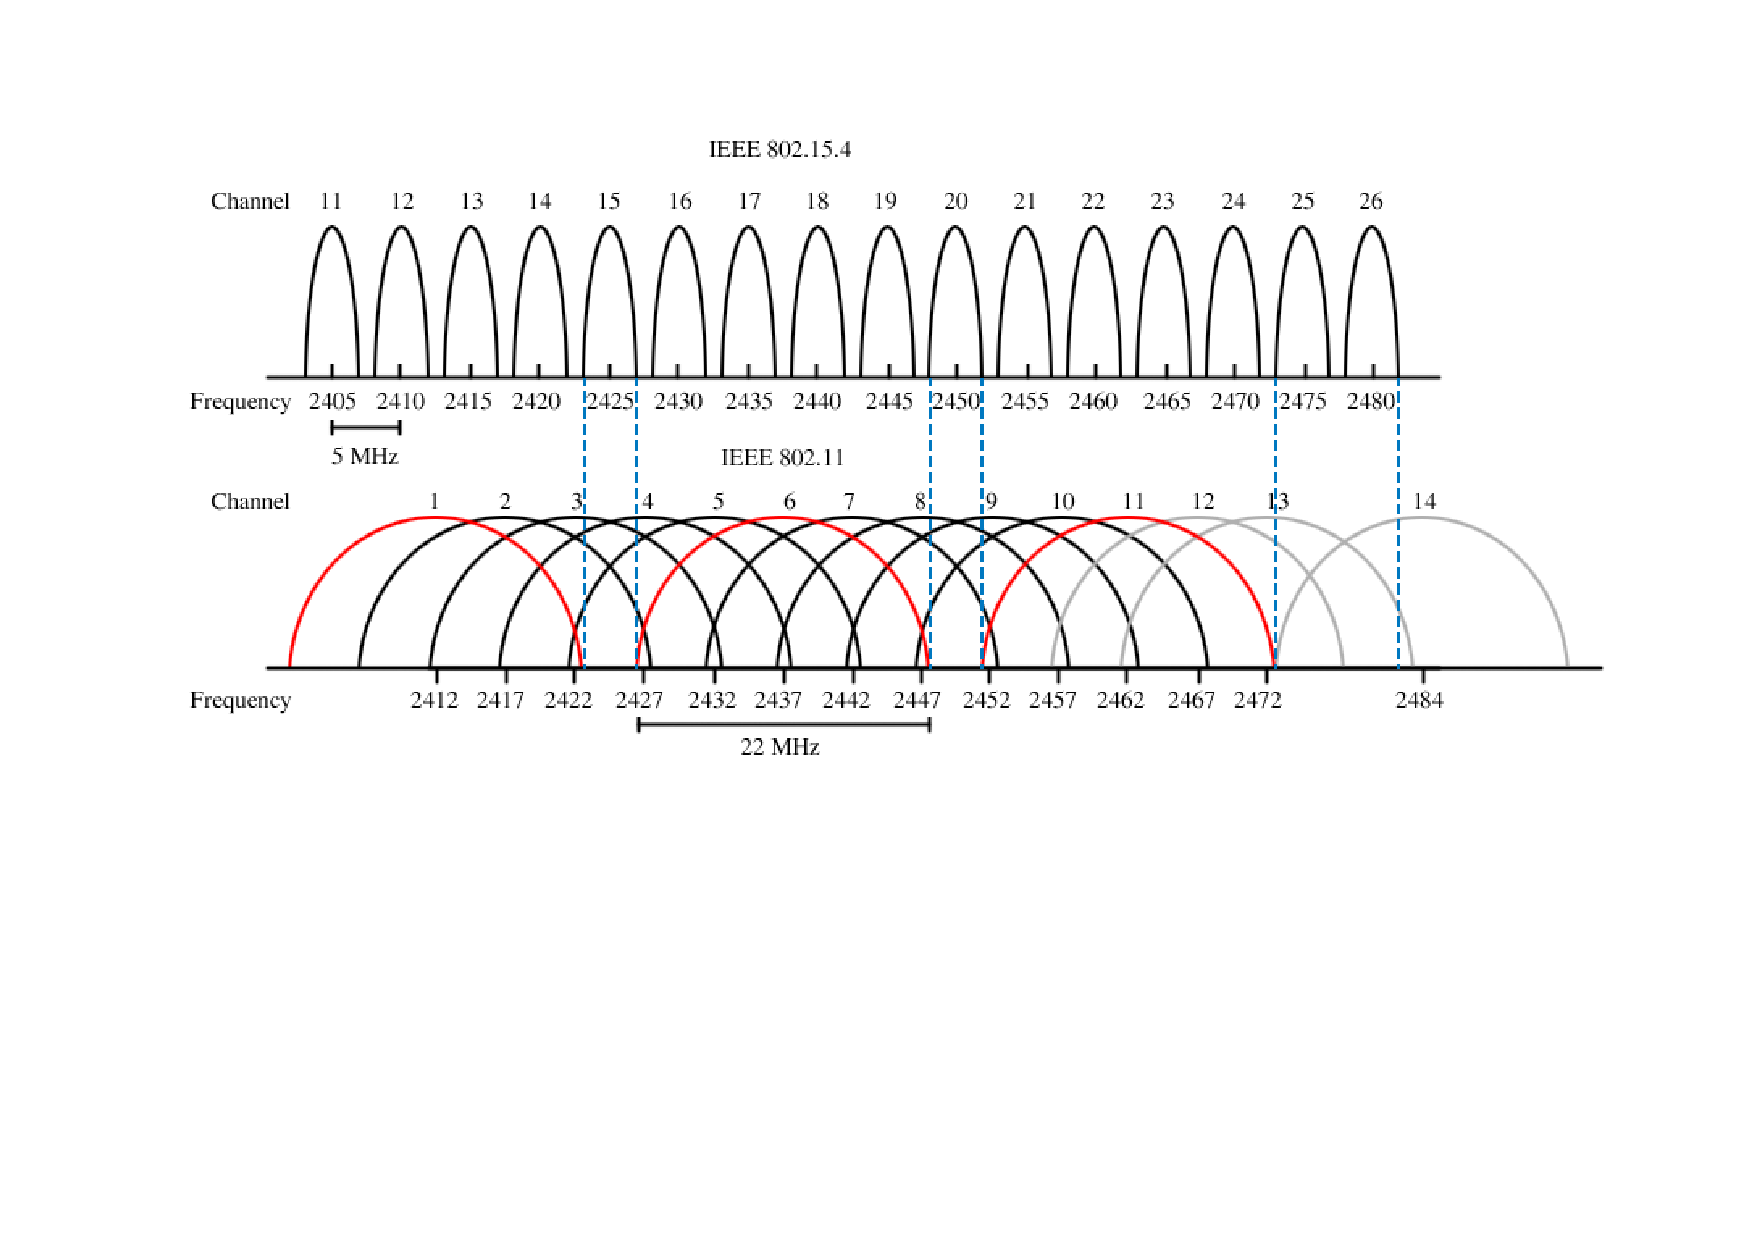
\includegraphics[trim=3cm 8cm 2cm 2cm, clip=true, width=0.45\textwidth]{figures/freqBand.pdf}
%\caption{IEEE 802.15.4 and IEEE 802.11 frequency channels in the 2.4 GHz ISM band}
%\label{fig:freqBand}
%\end{figure}

Upon start up, all nodes are initialised to channel 26 as it does not overlap with Wi-Fi. 
%which does not overlap with the Wi-Fi channels. 
%Channel 15, 20, 25 and 26 do not overlap with Wi-Fi as shown in Figure \ref{fig:freqBand}. 
%However, channel 26 is the selected clear channel based on the channels occupancy tested in three different locations; residential, public area and university (UCL) environments shown in Figure \ref{fig:interference2} where the figure shows only several selected signals. 
The environment condition and the network could be different depending on the location, time and channel occupancy. 
The authors in \cite{homearea} studied the channels reliability in residential areas in several neighbourhoods in comparison to an office (university) environment to show that the spectrum usage may be very different.
%as office environments are typically centrally managed. 
The authors in \cite{oppcast} showed similar results of different spectrum usage when comparing the interference patterns in offices (universities), public areas (shopping malls) and residential environments.
%This is proved in the hardware performance evaluation section by considering different environments in our experiments.
This shows that it is extremely difficult to find a good interference free channel and it varies from one location to another.

%\begin{figure}
%\centering
%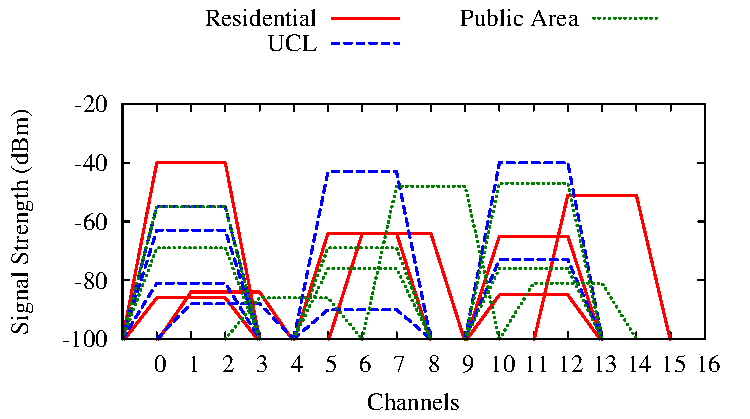
\includegraphics[width=0.45\textwidth]{figures/interference.pdf}
%\caption{Interference level on the channels at different locations}
%\label{fig:interference2}
%\end{figure}

The nodes will only be on the same channel (channel 26) once during the initial setup.
This enables the node to detect and find nearby neighbours that are in range to allow RPL set up mechanism to form the initial optimised topology before channel assignments can take place which improves the tree.
%before it can decides on the best route based on the list of neighbours it can be connected to.
%The usual RPL set up mechanism is used to exchange control messages that are required to form an optimised topology before channel assignments can take place.  
The initial channel should not be used as the transmission channel throughout the runs unless MCRP fails or could not find a better channel in order to not overload the initial channel.
%thus, the change to another interference free or low interference channel. 
It could lead to interference between the nodes competing for transmissions opportunity which is the problem in a single channel network. 
%To ensure reliable communications, two-hops colouring algorithm is used in channel selection to avoid the selected channel from overlapping with the other nearby transmissions.
%Two-hops colouring algorithm ensure reliable communications as the channels do not overlap during transmissions.

\subsubsection{Channel Selection Strategy}
One main advantage of the proposed system is generality. Any algorithm can be used at the LPBR to assign channels. MCRP uses a two-hop colouring algorithm to select a channel to be assigned to a node.
The two-hop colouring algorithm attempts to ensure that nearby nodes do not communicate on the same channel and risk interfering with each other. This enables simultaneous transmissions and allows fair load balancing on the channels. The protocol is inspired by the graph colouring problems \cite{graphColouring}. The core idea is that no node should use the same listening channel as a neighbour or a neighbour of a neighbour (two hops).
%%This allows fair load balancing on the channels and reduces channel interference that could occur when two nearby nodes transmit together on the same channel. 
%%To ensure reliable communications, two-hops colouring algorithm is used in channel selection to avoid the selected channel from overlapping with the other nearby transmissions.

%The nodes used in this experiment have a transmission range of approximately 20-30 metres indoors and 75-100 metres outdoors \cite{telosb-datasheet}. It could be the case that many nodes in a sensor network are in the transmission range of each other and potentially interfered with.

%All nodes are initialised to channel 26 which is the common default channel for Contiki MAC layer since it often has fewer interference problems with Wi-Fi and other sources. The studies in \cite{chrysso, micmac, watteyne} use a set list of whitelisted channels in their experiments and have channel 26 in common.
%However, the initial channel should not be used as the transmission channel throughout the runs (unless all channels check fail) in order to not overload the initial channel, thus, the change to another interference free or low interference channel. It could also lead to interference between the nodes competing for transmissions opportunity which is the problem in a single channel network. 

%Two-hops colouring algorithm ensure reliable communications as the channels do not overlap during transmissions.

%The usual RPL set up mechanism is used to exchange control messages that are required to form an optimised topology before channel assignments can take place. The nodes will only be on the same channel once during the initial setup.
%This enables the node to detect and find nearby neighbours that are in range before it can decides on the best route based on the list of neighbours it can be connected to. 

In the two-hop colouring algorithm, the LPBR chooses a node $N$ to which it will assign a new channel $D$ to listen on.
%The selection is random (from channels 11 to 26) based on the full range available \cite{ieee802.15.4}. 
Instead of checking all or several channels, MCRP chooses a random channel and learns the channel condition from the current run. 
The authors in \cite{energyluca} proposed a spectrum sensing algorithm to decide on the number of channels to be sensed before the channel is selected for transmissions. While it was found that sensing more channels increase the likeliness to find the best channel with less or no interference, it requires higher energy consumption and longer time delay during each check. 
%%%In the studies, three cases were considered where (i) all channels are sense, (ii) the energy consumed (channel conditions) in all channels are known and (iii) in the case where an energy threshold is set in unknown conditions. 
%While the studies showed selecting a channel from several channels check would give better chances of successfully transmit packets, it comes to the cost of energy and require longer period to check several channels.

%Instead of checking all or several channels, MCRP chooses a random channel and learns the channel condition from the current run. 
%The channel condition might vary depending on the location and time, and it could be the case where the same channel has different interference level each time. 
%However, knowing the channel condition does not have any benefit and require all or several channels to be rechecked each time. This consumes a lot of energy during each check. 
MCRP only considers two channels at a time, whether the new channel $D$ has better reception rate than the current channel $C$. By doing so, the channel selection is more spread out (random and fulfil two-hops rule) rather than all nodes trying to use the same best channel.
%The channels that were tested to have severe interference for one node might gives good result for another node depending on the location of the node which might not be within the range of where the channel has severe interference previously. 
%MCRP has its channel quality checking mechanism before it decides on a channel.
The protocol checks the node $N$ neighbours and neighbours of neighbours to see if any of those are currently listening on the selected channel $D$. If any are, a new channel $D$ is randomly chosen from the remaining list of available channels. 
%If the LPBR has knowledge of existing bad channels then those channels can be blacklisted.  
%%%Knowledge of channel interference which is gained by probing can be used to decide that a channel should not be used. If a channel is found then the channel switching protocol is triggered. 
%%???MCRP has its channel quality checking mechanism before it decides on a channel.
If no channel $D$ can be found meeting these conditions, the current channel $C$ is kept. 

The node selection algorithm must only attempt one channel change at a time to ensure probing is done on the correct new channel $D$ and for the node $N$ to finalise the channel to be used before another node attempts a channel change.
The protocol ascertains that the channel change attempt will always result in a message returned to the LPBR either confirming the new channel $D$ or announcing a reversion to the old channel $C$. Until one or other of these happens, no new channel change will be made to ensure that the neighbours are transmitting on the correct channel.

\subsubsection{Channel Switching}

\begin{figure}
\centering
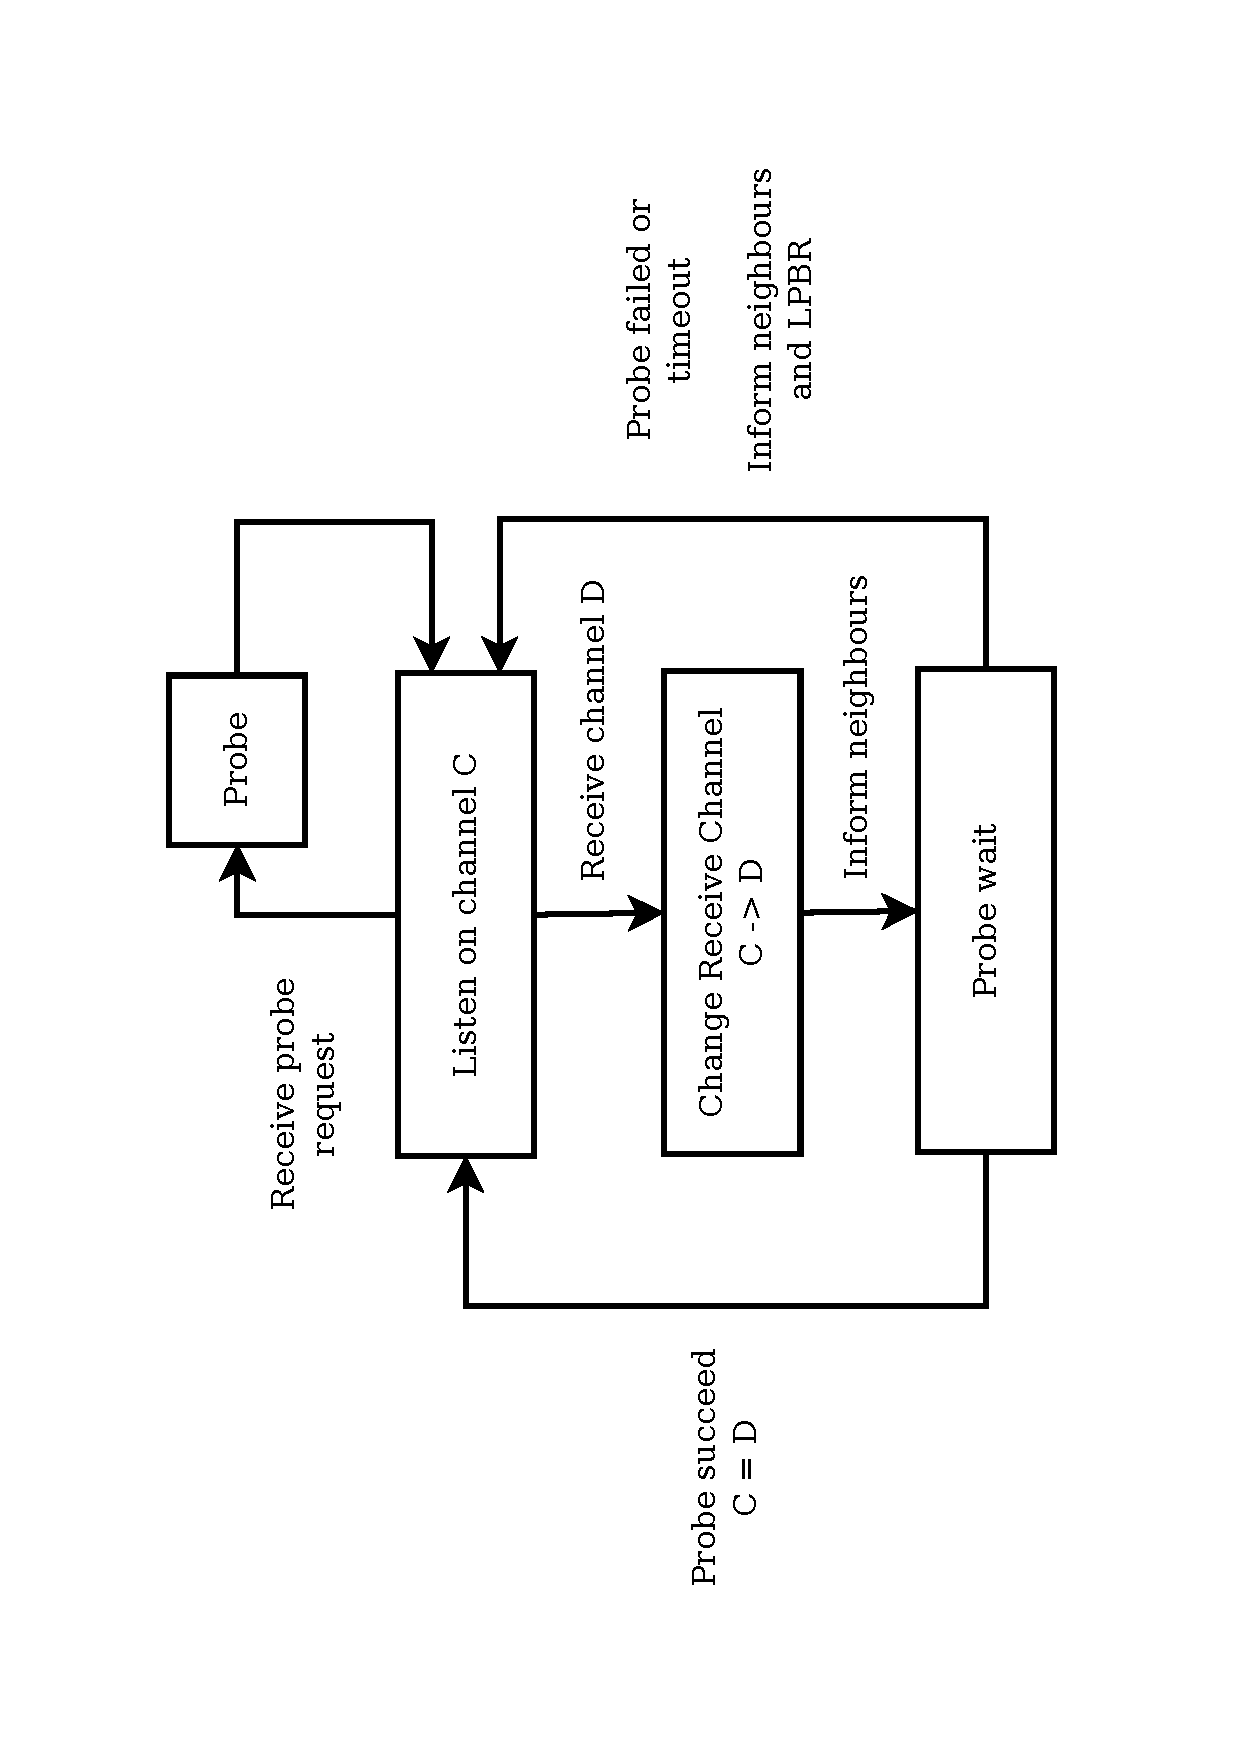
\includegraphics[trim=2cm 2cm 2cm 2cm, clip=true, totalheight=0.36\textheight, angle=270]{figures/channelSwitching.pdf}
\caption{MCRP processes}
\label{fig_mcrpDiagram}
\end{figure}

%Figure \ref{fig_mcrp} shows the state machine for the channel switching protocol.
As explained in the previous section, a choice of a new channel by the channel selection protocol causes the change channel message to be sent to the appropriate node. Figure \ref{MCRP} shows the steps in the protocol.
Upon receiving the channel change message, the node $N$ stores its current channel $C$ and communicates to all its neighbours the new channel $D$ that it wishes to change to. Those neighbours will update their neighbour tables to ensure that they now send to node $N$ on channel $D$.  The node $N$ begins the channel quality checking process with each neighbour in turn by sending them a probe request. If this process fails for any neighbour then the node reverts to channel $C$. Node $N$ informs its neighbours of the decision. The neighbours will update their neighbour table to transmit on channel $C$. If all channel quality checks succeed, the node $N$ will listens on channel $D$. Node $N$ does not send a confirmation message to the neighbours as it would be redundant since the neighbours already know the node $N$ listening channel. 
%In both cases, LPBR is informed of the channel checking results. LPBR updates the node's channel on its table.   
%In both cases, node $N$ informs its neighbours of the decision to channel $C$ or $D$ and informs the LPBR of the channel checking results. 
%%The channel checking process uses probe packets that might interfere with other transmissions temporarily. However, it is important to emphasise that the network remains fully functional and connected at all stages of this protocol.

\subsubsection{Channel Quality Checking}
Probing is essential to make the channel change decision. It gives a quick overview of the channel condition based on the number of probing messages received. The probe packets might interfere with other transmissions temporarily. However, it is important to emphasise that the network remains fully functional and connected at all stages of this protocol.

Probing is only done between the node $N$ and the tree neighbours. Tree neighbours are the nodes that a node does transmit to through the topology formed by the RPL protocol. The tree neighbour node is selected from the list of available neighbours based on the ability to transmit to the next hop towards the LPBR depending on the RPL. By default, it is decided by using the least expected number of transmission from the node to LPBR. Node neighbours are all nodes that a given node knows it could transmit to. The nodes are within the transmission range of each other.
%In describing the channel quality checking process, it is worth emphasising the distinction between neighbours and tree neighbours.  
Neighbours that are not tree neighbours will not use the node as a route during their transmission thus, there is no need for probing to take place with those neighbours. However, the neighbours still need to know the channel value given that RPL control messages are sent to neighbours directly without using the routes.

The channel quality checking is invoked each time a node $N$ changes channel after receiving a message from the LPBR. 
%The node $N$ changing to channel $D$ informs all neighbours in turn, of the new channel $D$ it will be listening on as described in the previous section. 
It then enters the \emph{Probe Wait} state and begins channel quality checking with each tree neighbour in turn. 
In the \emph{Probe Wait} state, node $N$ sends a \emph{Probe} message to each tree neighbour in turn. The neighbours respond to the message by sending eight packets to $N$ on the new channel $D$. 
The buffer can accommodate eight packets at a time. As the packets might not be sent immediately due to wakes up and collisions, sending more packets would have the risk of being dropped. The authors in \cite{homearea} observed that a short period of time is sufficient to give an overview of the channel condition as increasing the period shows minimal benefit.
The condition of the channel $D$ is further investigated through the number of retransmissions and packet collisions of the probing packets for accuracy of the channel condition. 

If the probing process times out (because of some communication failure) or the number of probe packets received is above a threshold (currently set to 16, including retransmissions and collisions) then node $N$ immediately exits \emph{Probe Wait} state and reverts to channel $C$ its previous channel. 
All neighbours are informed of the change back to channel $C$.
%and the LPBR is informed of the quality check failure with a summary of all probes received.
If, on the other hand, all channel quality checks succeed, the change to channel $D$ becomes permanent for node $N$.
In both cases, the LPBR is informed of the results with a summary of all probes received and the channel.

\subsubsection{Reconnection Strategy}
RPL routing protocol functionality remains the same. RPL control messages are adjusted to support multichannel.
%\cite{routingmetrics, winter2012rpl}.
%RPL topology could change according to the routing metric \cite{routingmetrics} the way the usual RPL would work \cite{winter2012rpl}. 
The nodes can still change the parents as usual as all neighbours are informed of any channel changes.
%for the nodes that are within the transmission range of each other.
%know each other new channels. 
%The neighbours that are not part of the route do not probe the parent when making the channel decision. However, the neighbours are informed of any channel changes.
This enables the topology to be optimised when communication fails and further improved through MCRP as the nodes have knowledge of the listening channels of all other nodes within the range. If a new node tries to join the topology, it sends a RPL control message through all channels as the listening nodes are unlikely to be on the initial channel. The new nodes will start on channel 26.
The listening nodes send a broadcast on the default channel to discover new nodes and send RPL messages through unicast when the neighbours are known to reduce unnecessary transmissions in broadcast on all available channels. New nodes and nodes which fall off the network can now rejoin on many potential channels.

%\subsubsection{Summary}
%This chapter introduces MCRP, a multichannel cross layer routing protocol that jointly optimise the network communications through channel decisions from the application, network and MAC layers. It uses a centralised controller for nodes channel allocation. The channel condition is tested through probing packets during run time as it varies depending on the location, time and usage. By doing so, the nodes would use less interference channels for communications to maximise the packet reception rate. MCRP uses a two-hop colouring strategy to avoid nearby nodes from competing to transmit on the same channel at the same time and internal interference that could occur. In order to allow reconnection and new nodes to join an existing topology, RPL control messages are adjusted to support multichannel. 